\documentclass{article}

% document settings
\usepackage{EngReport}
\geometry{letterpaper, portrait, includeheadfoot=true, hmargin=1in, vmargin=0.8in}
\renewcommand{\familydefault}{\rmdefault}

\usepackage{graphicx}
\usepackage{caption}
\usepackage{hyperref}

\begin{document}
\renewcommand{\familydefault}{\rmdefault}
\pagestyle{fancy}
\fancyhf{}
\setlength{\headheight}{25pt}
%\renewcommand{\headrulewidth}{0.4pt}
\renewcommand{\footrulewidth}{0.4pt}
\lhead{\normalsize Natural Language Processing \\ 31 March 2024}
\rhead{\normalsize Emma Franchino \\ Jingyi Zhang}
\rfoot{\textbf{Page \thepage}}
\lfoot{}

\fontsize{11}{15}\selectfont{
    \begin{flushleft}
    {\fontsize{16}{18}\selectfont\textbf{Exercise Three: Text Emotion Recognition}} 
\end{flushleft}

\section{Introduction}
For this project we chose to explore a field that results complex for both humans and NLP: emotion recognition. The task of recognizing emotions has always been highly interesting for the field of psychology, as well as conflictive: it’s hard to collect human emotions into categories, and even more to infer them from a text. This is what Text Emotion Recognition is trying to do: analyze sentences in order to detect the specific emotion that, for instance, a person writing  a comment on Twitter or YouTube was feeling at that moment. 

As a psychology student I find this a really hard task, especially if we haven’t a face or a speech tone to associate that text to; but at the same time a really intriguing NLP task, too. Thus, in this exercise we wanted to see if we were able to find a language model that could have a good accuracy in labelling some text with basic emotions, as well as detect the efficiency of a sentiment analysis, which is trained just on the distinction of positive and negative feelings, in two different languages, with a more complex differentiation of labels. 

Seeing the complication of this task we expect to find some difficulties in training a model with a high accuracy, as well as to detect a lower accuracy of the sentiment analysis compared to the one of the model.

\section{Material and methods}
We borrowed the language data from an emotion recognition task on \href{https://www.kaggle.com/datasets/parulpandey/emotion-dataset/code}{Kaggle}. The dataset consists of 2000 English sentences labelled from 0 to 5, each representing a distinct emotion. These sentences express emotion from a first-person perspective, and most of them start with “I feel”. The data was structured into two columns: “text” and “label” and stored in a CSV file. In addition, we translated these sentences into Italian with the same labels attached, to test it later with an Italian Sentiment Analyzer. 

In the original task, the author used a pre-trained BERT model for classifying emotions in tweets across multiple classes. We decide to apply two different approaches: first, applying the spacy module, which allowed us to  calculate the similarity between the label and the sentence (after trying with other more appropriate models such as Word2Vec or transformers, without succeeding); second, applying sentiment analysis using the VADER model, defining the values of the 0 to 5 categories.
For our Italian data, we will use the FEEL-IT model, which is an emotion and sentiment classification for the Italian language provided by Hugging Face. 

After performing the emotion prediction, we will examine the model accuracy and compare it to the baseline accuracy. Since the FEEL-IT model only has 4 labels that are included by the 6 of our data, we will have to adapt our considerations of the accuracy of the model to this. \\
We also need to mention that this sentiment analysis will take a long time to make the predictions when running the code, but the outputs can be easily found in the file "predictions\_FEEL-IT.txt".

\section{Results}
In the original count of the 6 emotions, we found that joy appears to be the most frequent, followed by sadness, anger, love, fear and surprise ({Figure \ref{fig 1: original dataseet}}). By comparing the original counts and the predicted counts of emotion, we will value the model quality. We assumed that since most sentences are structured in a plain way to express emotion (“I feel…”), the prediction shall be quite easy.

The first outputs we evaluate are the ones generated by the similarity, where we encountered almost every prediction as “sadness” ({Figure \ref{fig 2: similarity model}}), and with an accuracy of 0.2895. Obviously here the model didn’t work as we expected, and we found some serious difficulties in understanding which was the problem, especially because “sadness” is not even the most frequent label in the original dataset. 
We analyzed the problem deeply, getting to the conclusion that calculating the similarity is not the best choice for this kind of dataset, since the results are always low between a label and a long sentence, with a higher value for the word “sadness”. We tried to improve the accuracy with other methods such as using transformers and models like “Word2vec” and “sense2vec”, but couldn’t manage to get to the results. 

We then tried to make predictions of the emotions labels with pre-trained models for sentiment analysis, we firstly used was VADER, here our results showed an accuracy of 0.3395, which is pretty low, just below the baseline. This result can be seen in the frequency of the labels in {Figure \ref{fig 3: VADER model}}.
Specifically, we found the prediction for joy, love and anger are close to the original counts, while for sadness, fear and surprise are not very accurate. We assume that since the sentiment analysis is categorized based on the positive/negative distinction, the emotions that fall on the polars (joy and love: positive, anger: negative) are easier to be detected, while the rest are more neutral and harder to define. Plus, some contexts being semantically ambiguous may also cause an influence.

Lastly, we tested our dataset in another language: Italian, using another pre-trained sentiment analysis model, created for this language, called “FEEL-IT”. The results of this model can be seen in {Figure \ref{fig 4: FEEL-IT model}}. We have to take into account that only four types of emotion are predicted in this model. We found the prediction for joy, anger and fear obtained impressively close counts to the original, and we attribute the success to the model training. We assume that surprise and love counts were assigned to sadness, which leads to its high count value. It could be due to the similar reason above: that these two emotions are less polarized. Sometimes surprise or love can just be sad. 
While this model deals with the Italian translation of our data, the syntax structure remains almost the same; and the meanings are unchanged. Therefore, we do not see it as a flaw.

In summary, the FEEL-IT model yields the highest prediction accuracy, followed by VADER and similarity models. In particular, “surprise” seems to have the most errors to predict for all three models, which might be due to its less frequent appearance in the data as well as the semantic ambiguity. 
The limitations of the models we used are many, from the similarity of one not being adapted for this kind of task, to the number of categories of the FEEL-It model and the overall low accuracy of the VADER model.
Despite being aware of the many limitations that we encountered, we think that this displays also the complexity of the task, which is affected by many variables of the dataset, too;  and the difficulties in recognizing human emotions by machines (reflected by humans themselves, too). 

\section{Code}
The Python code used to analyze the data can be found \href{https://github.com/emmafranchino/nlp_assignments/blob/main/exercise_three/ex_three.ipynb}{here.}\\
The dependencies that need to be fulfilled to run the code are:\\
- matplotlib.pyplot as plt \\
- numpy as np \\
- pandas as pd \\
- spacy \\
- from transformers import pipeline \\
- from collections import Counter \\
- nltk \\
- from nltk.sentiment.vader import SentimentIntensityAnalyzer

\section*{List of contributions}
Emma, being a psychology student, worked more on the idea of the task and the Introduction. Jingyi focused more on the methodology part as well as the sentiment analysis; instead Emma focused on the similarity model. 
Both of us worked together to overcome problems and difficulties during the coding part and the writing of the results section. 
}

% \newpage
\section*{Figures}
\begin{center}
    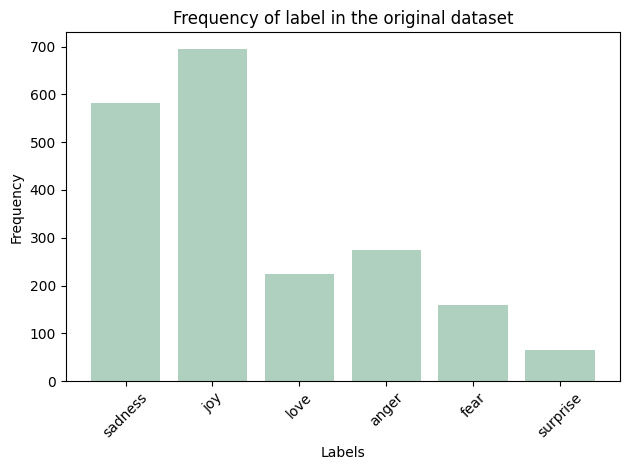
\includegraphics[width=0.8\textwidth]{./figures/fig_1.png}
    \captionof{figure}{Frequency of emotion labels in the original dataset}
    \label{fig 1: original dataseet}
\end{center}

\begin{center}
    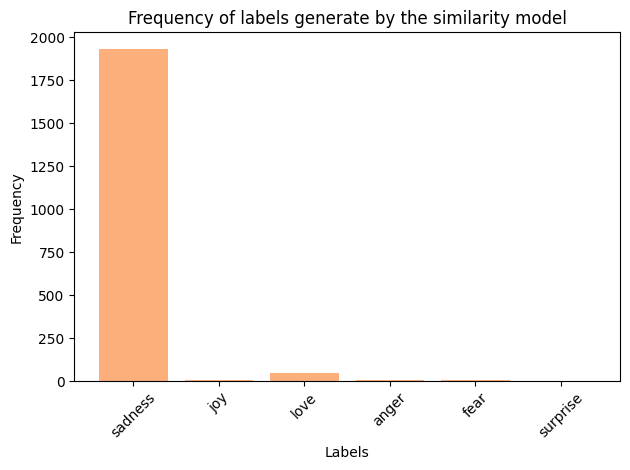
\includegraphics[width=0.8\textwidth]{./figures/fig_2.png}
    \captionof{figure}{Frequency of emotion labels generated by the similarity model}
    \label{fig 2: similarity model}
\end{center}

\begin{center}
    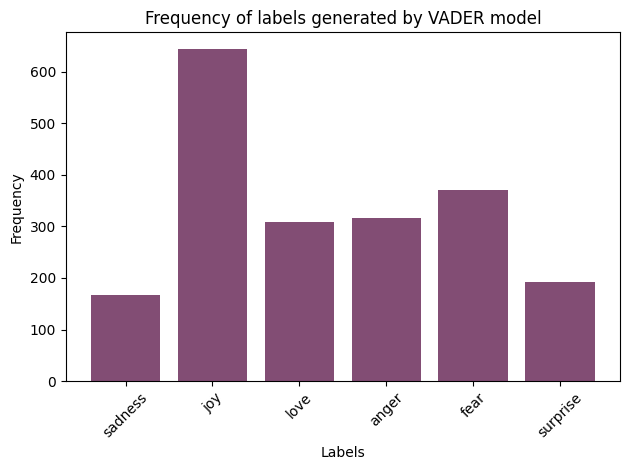
\includegraphics[width=0.8\textwidth]{./figures/fig_3.png}
    \captionof{figure}{Frequency of emotion labels generated by VADER model}
    \label{fig 3: VADER model}
\end{center}

\begin{center}
    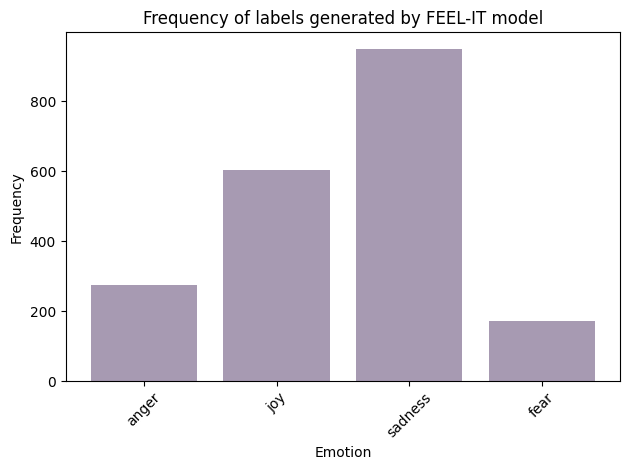
\includegraphics[width=0.8\textwidth]{./figures/fig_4.png}
    \captionof{figure}{Frequency of emotion labels generated by FEEL-IT model}
    \label{fig 4: FEEL-IT model}
\end{center}

\end{document}
